% =====================================================================
%  Literature Review
% =====================================================================

\chapter{Literature Review}
\label{sec:litReview}

% ---------------------------------------------------------------------
\section{Wind Measurement in the Wind Energy Sector}
    \subsection{Introduction}
    Wind has become a mainstream source of electricity. A record 165\,GW of
    new wind capacity was installed worldwide in 2025, 40\% more than the
    previous record year, bringing cumulative capacity to roughly 1.3\,TW
    across 138 countries \cite{gwec2026}. Delivering that growth at acceptable cost depends on how well the wind
    resource itself can be characterised, which Veers et al. identify as one
    of the grand challenges of wind energy science \cite{veers_grand_2019}.
    Wind speed is an important factor in analysis of a turbine's economics
    and engineering. The power available in the wind scales with the cube of
    wind speed, so a small error in measured or predicted wind speed becomes
    a much larger error in predicted energy \cite{windenergyhandbook}. Furthermore, wind speed and turbulence significantly affect the structural fatigue on a turbine, and act as an input to controllers which control the pitch and yaw of the turbines appropriately to maximise power generation and minimise stresses on the structure. It is clear that real-time measurement of the wind field around wind-turbines is a critical objective for this industry, and one to which much attention must be given. However, turbines operate in the lower atmospheric boundary layer, where the flow
    is turbulent and shaped by mesoscale circulation, orography, thermal stratification and the wakes of neighbouring turbines, which makes this characterisation of the wind-field difficult \cite{letizia_characterization_2023}.
    

    \subsection{Current In-Situ Anemometry Methods and Limitations}
    The traditional instrument for wind-speed measurement for wind-turbines is the meteorological mast (met-mast),
    which holds cup and sonic anemometers at fixed heights, mounted on a long mast. This technology is well established, providing high resolution measurements, and indeed acting as a reference point to which any alternative method is compared \cite{liu_review_2019}, \cite{hill_remote_nodate}. This methodology however holds several limitations:

    Erecting a meteorological mast can be costly, particularly for offshore wind-turbines \cite{wagner_uncertainty_2016}. Once constructed, the  met-mast is naturally limited to a single location, which limits spatial coverage - this makes variability in the wind, which occurs over larger areas, difficult to characterise \cite{letizia_characterization_2023}. Furthermore, the wake of the mast itself can corrupt measurements in the anemometer \cite{letizia_characterization_2023}. These constraints motivated the research into a remote sensing alternative to in-situ measurements.
    
    
% ---------------------------------------------------------------------
\section{LiDAR as an Alternative}

    \subsection{Introduction}
    Advancements in LiDAR technology have resulted in the technology presenting an alternative and/or complement to existing wind-speed measurement techniques. This allows for the development of new turbine control and assessment strategies, which overcome some of the limitations of traditional wind-speed measurement techniques. 

    Doppler wind LiDAR (DWL) systems measure the line-of-sight velocity of wind by emitting a laser beam into the atmosphere and measuring the Doppler shift of the beam after being backscattered by naturally occurring aerosols and particles (see \autoref{sec:lit-principlesDWL}). There are numerous commercial DWL systems available, such as Qinetiq's ZephIR whose first deployment was on the nacelle of a 2.3\,MW turbine, and with Vaisala's (formerly Leosphere) pulsed WindCube shortly afterwards \cite{hill_remote_nodate} \cite{cariou_leosphere_nodate}. Research has been focused on two areas; ground-based systems for wind-speed measurement (primarily for resource assessment prior to building wind-energy farms), and nacelle-mounted LiDAR (NML) systems \cite{letizia_characterization_2023}. 
    
    Letizia et al. identified several promising application areas for NML systems, including load reduction, performance optimization, and performance assessment \cite{letizia_characterization_2023}. NML systems present several advantages over traditional measurement techniques for these ends, including larger field of view and spatial coverage (particularly for scanning LiDARs) and reduced costs and maintenance \cite{letizia_characterization_2023}. The following subsections provide a brief overview of different NML application areas, and progress and limitations in these sectors. These areas of research present viable means to lower the levelized cost of energy (LCOE) for wind-turbines, and are thus well-suited to the growing demands for wind-energy systems globally \cite{letizia_characterization_2023}. 

    \subsection{NML for Load Reduction}
    Wind gusts can place significant load on a wind-turbine structure - however appropriate control of the turbine's rotor pitch can serve to decrease this load, preserving the structural integrity and longevity of the system.
    Standard turbine controllers are feedback systems that react to
    a turbulent gust only after it has loaded the rotor. A lidar preview of
    the approaching wind-field however would enable feed-forward pitch action \textbf{before} the gust
    arrives, and there is consensus that load reduction in certain regions of wind-turbine operation is a promising lidar-assisted control
    (LAC) application \cite{letizia_characterization_2023}. Crucially however, any benefit from feedforward LAC for load-reduction is limited by
    the coherence between the wind-speed measured by the LiDAR from a distance, and the actual wind-speed which hits the turbine rotors (rotor-effective wind-speed) \cite{letizia_characterization_2023}. The seminal simulation study of Harris et al. reported a 10\% reduction
    in damage-equivalent load on the flapwise blade root \cite{harris2006}, which spurred on further research into the topic. There is much ongoing research on the topic, particularly with respect to the evolution of the wind-field in between sensing and reaching the turbine, and reported results span a wide range. This lack of consolidation has thus presented a barrier to widespread adoption of LAC for load reduction, however research thus far indicates that this is indeed a promising application of the technology \cite{simley_optimizing_2018} \cite{letizia_characterization_2023}. 
    
    \subsection{NML for Performance Optimization}
    Another application area for LAC is performance optimization, where feedforward control based on NML measurements of the incoming wind-field can be used to yaw and pitch the turbine appropriately, and use torque control to maintain optimal rotor speed, so as to maximise power generation. This has however showed limited results in comparison to load reduction. Simulation studies thus far have found negligible gains in power coefficient from feed-forward torque control for optimising rotor speed, because conventional non-LAC torque controllers are already
    mature \cite{letizia_characterization_2023}. Where gains are reported they come from yaw correction - a
    hub-mounted ZephIR used to correct misalignment on a 2\,MW turbine gave
    an estimated 5\% annual energy production increase \cite{letizia_characterization_2023}. 
    
    \subsection{LiDAR for Performance Assessment}
    Power performance testing is an area in which NML has had greatest success and widespread adoption \cite{letizia_characterization_2023}. A turbine's power curve is conventionally
    measured against a met-mast's wind-speed measurements. Mikkelsen et al. used a spinner lidar (mounted on the wind turbine blades rather than the nacelle) to reconstruct the low-speed end
    of a 2.3\,MW turbine's power curve and found less scatter than the met-mast
    measurement, which they attributed to a more representative
    rotor-equivalent wind speed \cite{mikkelsen_spinner-integrated_2013}. Wagner et al. achieved similar results, and identified the reasons:
    because the lidar yaws with the turbine it always measures upwind, so
    its measured wind-speed correlates better with power fluctuations than the met-mast's; and
    because it is never in the wake of the turbine under test, the usable wind sector was larger than the undisturbed sector of the cup
    anemometer \cite{wagner_power_2014}. This shows a direct advantage of a DWL system over traditional in-situ measurements, where the met-mast is fixed. A subsequent uncertainty analysis found
    the NML estimated annual energy production only 1.1\% more uncertain than the cup-anemometer reference, its
    higher instrumental uncertainty offset by greater data
    availability \cite{wagner_uncertainty_2016}.
    The International Electrotechnical Commission (IEC) formalised the method in 2022 \cite{iec61400-50-3}, and some 500 campaigns
    per year are projected this decade~\cite{letizia_characterization_2023}.
    
    \subsection{Discussion of NML Applications}
    The three application areas discussed above present results which show some of the use-cases of LiDAR for wind-speed measurement, however they are not exhaustive, and the topic remains an active area of research. What is however clear in the literature is that the widespread adoption of such systems depends on the reliability, accuracy and cost of the LiDAR systems \cite{letizia_characterization_2023}. Traditionally, such systems have been very expensive, and there has been research into methods to reduce the cost \cite{bennett_doppler_2003}. The remainder of this report thus addresses aspects related to the design of such systems, and the costs and tradeoffs involved. 
% ---------------------------------------------------------------------
\section{Principles of Doppler Wind LiDAR}
\label{sec:lit-principlesDWL}
% Lead-in: single continuous physics narrative from here to the end of
% the section -- no application material interleaved.
Doppler wind LiDAR uses a simple working principle in order to determine wind-speed from a distance. The following section details the physics and mathematical concepts which are used in DWL systems.

    \subsection{Aerosol Backscatter and the Doppler Shift}
    % Mie scattering from ambient aerosol; f_D = 2 v_r / lambda;
    % origin of the factor of two.
    LiDAR systems emit very high-frequency electromagnetic radiation (when compared to its technological cousin - radar), thus, wavelengths of the emitted radiation will be very small. This property makes the technology uniquely suitable for the purposes of wind-speed measurement; the wavelength of the emitted LiDAR beam is comparable to the size of the aerosol particles, and thus the particles scatter some of the emitted beam (Mie scattering) \cite{mikkelsen_spinner-integrated_2013}.
    
    The backscattered light can be detected by the LiDAR system's photodetector. The backscattered light, however, will be shifted in frequency relative to the incident LiDAR beam, by a magnitude which depends on the velocity of the particle itself - this is due to the Doppler effect \cite{Doppler1842}. Specifically, the shift in frequency of the backscattered light is directly proportional to the  line-of-sight (LOS) velocity of the particle - that is, the component of the particle's velocity in the direction of the line of the LiDAR beam - through the following equation \cite{letizia_characterization_2023}:

    \begin{equation}
        v_{LOS} = \frac{c}{2}\frac{f_{beam}-f_{scatter}}{f_{scatter}}
        \label{eq:DopplerShift}
    \end{equation}

    Note the factor of 2 in the denominator, which is necessary to account for the fact that the Doppler shift occurs twice - once for the emitted light hitting the moving particle, and again for the light being emitted/scattered \textbf{from} the moving particle. 

    Thus, by determining the Doppler frequency shift of the received backscatter from aerosol particles, the LOS velocity of those particles can be determined, and from this, the LOS wind-speed can be inferred. Note that this explanation simplifies concepts used in ranging of the wind-speed, which will be discussed in later sections. 

    \subsection{Challenges in Measuring Doppler Shift in DWL} \label{sec:lit-ChallengesDopplerShift}
    A crucial challenge in DWL is the measurement of the Doppler shift itself. LiDAR beam frequencies are of the order of
    $10^{14}\,\text{Hz}$ (hundreds of terahertz) while, from
    equation~\ref{eq:DopplerShift}, the Doppler shift in this THz-range signal, produced by
    aerosols moving at typical wind speeds is of the order of only
    $10^{6}\text{--}10^{7}\,\text{Hz}$ (a few megahertz) - this is a fractional frequency shift of
    roughly one part in ten million which needs to be resolved. Photodetectors can not follow typical LiDAR optical signals, which are in the order of THz. For example, for a LiDAR system with beam wavelength 1550 nm, the field oscillates at ~193 THz, orders of magnitude beyond the bandwidth of photodetectors or typical ADCs \cite{abari_all-fiber_2014, hill_remote_nodate}. Thus, the return backscatter signal's frequency can \textbf{not} be directly measured, and its frequency relative to the emitted beam simply observed from this. Instead, specialised techniques need to be used to recover the Doppler shift of the signal, \textbf{without} having to measure the frequency of the THz-range return signal for comparison. This is thus a central difficulty in DWL systems, and the detection architectures used to address it are discussed in the sections that follow.

        
    
    \subsection{LiDAR Detection Modes}
    LiDAR systems are typically grouped into two main types, each with their own distinct advantages, based on how received light is detected - these types are Direct Detection, and Coherent Detection. To varying extents, both of these detection modes have been applied in DWL systems, with significant differences in how the Doppler shift is measured in each. This section gives an overview of the principles of each detection mode, and discusses how this can be utilised to measure the Doppler shift of received backscatter light. 
    
    
        \subsubsection{Direct Detection}
        \label{sec:lit-directDetection}
        % Edge / fringe-imaging techniques; molecular vs. aerosol regimes.
        % Close with an explicit statement of why this branch is set aside.
        Direct detection LiDAR systems operate on a very simple principle: A laser pulse is fired from the system; this pulse then gets reflected off a target (or backscattered in the case of aerosols), and the reflection is incident \textbf{directly} on the LiDAR system's photodetector. Owing to its simplicity, direct detection LiDAR systems are widely used in robotics and automotive applications for ranging and basic velocity measurements. The time between the emitted pulse and received pulse can be used to calculate the distance of targets from the system, and repeated distance measurements can be used to estimate the velocity of the target. Obtaining velocity through Doppler shift measurements however presents a challenge to this architecture.
        
       As discussed in Section \ref{sec:lit-ChallengesDopplerShift}, photodetectors by themselves can not be directly used to determine the Doppler shift, as they can not follow THz frequency light signals. Multiple modified direct detection DWL system architectures have been developed to address this problem. Most common is the "double-edge technique" illustrated by Korb et al. \cite{korb_theory_1998}. Two Fabry-Pérot Interferometers (etalons) tuned symmetrically around the transmit laser frequency are used to split the backscatter signals - and thereafter the Doppler shift may be obtained from the ratio between the intensity of the two signals, as measured by photodetectors \cite{colberg_diode-laser-based_2026}. 
       
       Crucially for this method, the ratio between scattering types (Rayleigh and Mie) for the aerosols, as well as temperature must be known in order to produce accurate measurements - this can vary significantly with altitude \cite{werner_doppler_2005}. These factors, and strict requirements on etalon tuning, temperature, and laser stability present a considerable challenge in the implementation of this architecture \cite{colberg_diode-laser-based_2026}. In the double-edge technique any drift of the laser relative to the etalon edge is
        indistinguishable from a Doppler shift, so the transmit laser must be absolutely stable to roughly 100KHz of its nominal frequency, which in practice requires an active lock to an atomic transition \cite{colberg_diode-laser-based_2026}.
        The etalon itself must be temperature controlled to about 1 milli-Kelvin, since a 1 milli-Kelvin
        drift produces a $0.95m/s$ error, and mechanical drift of the mount can produce biases of $1.5-2m/s$ per week, requiring weekly recalibration \cite{colberg_diode-laser-based_2026}.
        
        An advantage that direct detection architectures hold over coherent detection is the ability to use molecular backscattering return (Rayleigh scattering), which gives it better performance in high-altitude regions with less aerosols to give particulate backscattering (Mie scattering, which a coherent detection system relies on) \cite{colberg_diode-laser-based_2026}. However, direct detection DWL systems typically have worse accuracy and spatial resolution than their coherent detection counterparts, which are more technologically mature \cite{werner_doppler_2005}. For these reasons, Direct detection architectures are not as common in the literature on DWL, as compared to coherent detection systems, particularly in typical wind-turbine applications in the aerosol-rich boundary layer, where the primary advantage of direct detection architectures is unnecessary. The remainder of this review will thus focus on coherent detection systems, and the intricacies of their system architecture. 
        

        \subsubsection{Coherent Detection}
        \label{sec:lit-coherentDetection}
        % Optical mixing with a local oscillator; beat signal; CNR;
        % shot-noise-limited operation and the LO power crossover condition.
        Coherent detection LiDAR varies from direct detection in that the return signal (from backscatter or reflections) is optically mixed with a local oscillator (LO) signal prior to detection. Typically, a single laser source is used, where a set fraction of the beam is emitted at the target, and the other fraction is used as the LO for mixing down the line. Coherent detection provides multiple distinct advantages over direct detection, which will be described in this section.

        Firstly, the optical mixing of the signals makes it possible to electronically distinguish a MHz-range Doppler shift on top of a THz-range carrier (as was identified to be a key challenge in DWL in  Section \ref{sec:lit-ChallengesDopplerShift}). This can be described mathematically as follows: If the laser source (and therefore LO) has frequency $f_0$, and the return signal has frequency $(f_0 + \Delta f)$, where $\Delta f$ is the frequency shift of the return signal due to the Doppler effect, the signal after mixing the return signal with LO is given by:

        \begin{equation}
            E_{mixed}(t) = \sqrt{2P_{LO}}\cos(2\pi f_{0}t)
                 + \sqrt{2P_{RS}}\cos(2\pi (f_{0}+\Delta f)t)
        \label{eqn:opticallyMixed}
        \end{equation}

        Where $P_{LO}$ and $P_{RS}$ are the time-averaged optical powers of the local oscillator and return signal respectively.
        
        The photodetector current, $I_{det}$, is proportional to the intensity of the  electromagnetic field of the light signal - $|E_{mixed}|^2$. When expanded, one obtains:
        
        \begin{equation}
        \begin{split}
            I_{det}(t) \propto\;
            &\underbrace{P_{LO} + P_{RS}}_{\text{DC}}
            \;+\; \underbrace{2\sqrt{P_{LO}P_{RS}}\cos(2\pi \Delta f\, t)}_{\text{beat}} \\
            &+\; \underbrace{P_{LO}\cos(4\pi f_{0} t)
                + P_{RS}\cos\!\left(4\pi (f_{0}+\Delta f) t\right)
                + 2\sqrt{P_{LO}P_{RS}}\cos\!\left(2\pi (2f_{0}+\Delta f) t\right)}_{\text{not followed by detector}}
        \end{split}
        \label{eqn:squared}
        \end{equation}
        
        It can be seen from the above equation that the squared mixed signal has three components: one at DC, one with frequency in the order of $f_0$, and another with frequency at $\Delta f$. Note again that $f_0$ is in the THz range, where $\Delta f$ is in the MHz range. As discussed, if a MHz-range bandwidth photodetector is used to detect $E_{mixed}$, the detector cannot follow oscillations at frequencies in the order of $f_{0}$, so those terms produce no response and may be omitted. Thus, \autoref{eqn:squared} simplifies to the following equation, which is called the beat signal:

        \begin{equation}
            I_{det}(t) \propto [P_{LO} + P_{RS}] + 2\sqrt{P_{LO}P_{RS}}\cos(2\pi \Delta f\, t)
            \label{eqn:beatSignal}
        \end{equation}

        Thus, if the frequency of this beat signal is measured, the Doppler shift, $\Delta f$, is obtained. In this way it can be seen that coherent detection allows for direct measurement of the Doppler shift, and therefore the velocity of the target. 

        Aside from the direct measurement of the Doppler shift, the "signal beating" process described above provides several other key advantages. The beating process amplifies the return beam, which allows for shot-noise limited operation (the ideal case for such a system), and extremely high sensitivies \cite{hill_remote_nodate} (elaboration in \ref{sec:lit-BalancedDetection}). This is essential in DWL, as return signals in clear atmospheric conditions are typically very low, due to low backscatter from aerosols. Furthermore, this detection process rejects signals which are not common in spatial mode and polarisation with the LO, meaning that sunlight, or other LiDAR beams will not affect the measurement \cite{hill_remote_nodate}. 
        

    \subsection{Coherent Detection: Homodyne, Heterodyne and Directional Ambiguity}
    \label{sec:lit-homohetero}
    
    % Zero-IF mixing and the sign ambiguity in the radial velocity.
    % Resolution options: acousto-optic frequency shifting, IF sampling,
    % image-reject (I/Q) architectures.
    % Close by stating which option is adopted and the accepted trade-off.
    The following section discusses two distinct classes of coherent detection methodology, and how the choice of class affects the recovery of the wind direction from the signal.

    \subsubsection{Homodyne}
    While not explicitly stated, the previously discussed direct down-conversion of the return signal to the beat signal - via mixing with a local oscillator with the \textbf{same} frequency as the emitted signal (\autoref{eqn:beatSignal} and preceding) - is known as \textbf{homodyne} coherent detection. Homodyne coherent detection down-converts the MHz-range doppler shift in the THz range carrier to a MHz-range beat signal around baseband, i.e. the frequency of the signal is directly the frequency of the Doppler shift. This has significant implications:

    Ignoring the DC components in \autoref{eqn:beatSignal}, we get
    %
    \begin{equation}
        I_{det}(t) \propto \cos\!\left( 2\pi \, \Delta f \, t \right).
        \label{eq:homodyne_beat}
    \end{equation}
    %
    The Doppler shift ($\Delta f$) therefore appears directly at baseband. However, because the
    cosine is an even function,
    %
    \begin{equation}
        \cos\!\left( -2\pi \, \Delta f \, t \right)
        = \cos\!\left( 2\pi \, \Delta f \, t \right),
        \label{eq:sign_ambiguity}
    \end{equation}
    %
    Therefore, noting that $\Delta f$ is signed based on whether the target is approaching or receding, it can be seen that approaching and receding targets of equal speed produce identical detector
    currents. Only the magnitude $\lvert \Delta f_D \rvert$ is recoverable, and the
    measured spectrum is symmetric about zero frequency. Note that Abari et. al\cite{abari_all-fiber_2014} demonstrated a methodology for obtaining signed velocity, even with a homodyne coherent detection setup, however this setup is novel and introduces additional complexities and costs which are outside of the scope of this project. 

    \subsubsection{Heterodyne}
    The alternative to this is known as \textbf{heterodyne} coherent detection. In heterodyne architectures, a slight frequency shift is imposed on the laser - crucially however this shift is only applied to one of the fractional outputs, either the local oscillator \textbf{or} the emitted laser (but not both). This means that when the same beating process described previously is applied, the MHz-range doppler shift in the THz range carrier is down-converted to a MHz-range beat signal centered around an intermediate frequency ($f_i$ below), rather than baseband, as with homodyne architectures. This is conventionally achieved with an
    acousto-optic modulator, placed either in the local oscillator arm \cite{harris_role_1998} or in the transmit arm \cite{abdelazim_development_2015}. This has the advantage of allowing for the recovery of the target's direction:
    
    Taking the offset in the local oscillator arm, such
    that $f_{LO} = f_0 - f_i$, the beat term becomes
    %
    \begin{equation}
        I_{det}(t) \propto \cos\!\left( 2\pi \left( f_i + \Delta f \right) t \right).
        \label{eq:heterodyne_beat}
    \end{equation}
    %
    Provided $f_i > \lvert \Delta f \rvert_{\max}$, the sign of $\Delta f$ is recoverable. Approaching targets appear above $f_i$ and receding targets below it, and the sign of the velocity is recovered.

    \subsection{Coherent Detection: Noise Sources and the Shot-Noise Limit}
    \label{sec:lit-noiseSources}
    In a coherent detection DWL system, there are four primary sources of noise which need to be considered, namely electronic noise, shot noise, relative-intensity noise, and phase-induced intensity noise:

    Electronic noise arises from the photodetector and the transimpedance amplifier (which converts photodetector current into a measurable voltage), and includes dark noise (signal present when there is no light incident on the detector) and thermal noise \cite{hill_remote_nodate}. This noise is constant, independent of LO power \cite{cariou_leosphere_nodate}, \cite{abdelazim_development_2015}. 

    Shot noise is a fundamental noise source in coherent detection. Shot noise arises from the discrete nature of photons, which reach the photodetector at slightly different random instants \cite{paschotta_shot_noise}, i.e. it is a property of light itself, and can therefore not be removed.  Because
    the photodetector's current is generated by these received photons, the detector then produces a white, Gaussian noise current whose power spectral density is
    proportional to the intensity of the light incident on it \cite{paschotta_shot_noise}. In the case of a coherent detection setup, it is thus proportional to $P_{LO}$. The significance of shot noise follows from comparing its scaling with
    that of the beat signal. From \autoref{eqn:beatSignal} the beat current
    has amplitude $\propto 2\sqrt{P_{LO}P_{RS}}$, so the signal
    power is
    proportional to $P_{LO}$. Shot noise power is also proportional to $P_{LO}$ \cite{cariou2006laser, abdelazim_development_2015}.
    Electronic noise power, however, as mentioned, is constant with $P_{LO}$. Neglecting other noise sources for the moment, the SNR is approximately
    \cite{cariou2006laser}:
    
    \begin{equation}
        \mathrm{SNR} = \frac{P_{LO} P_{RS}}
                            {P_{EN} + P_{SN}}=\frac{P_{LO} P_{RS}}
                            {P_{EN} + \alpha P_{LO}}
        \label{eqn:lit-SNR}
    \end{equation}

    Where $P_{EN}$ is electronic noise power, $P_{SN}$ is the shot noise power, and $\alpha$ is a proportionality constant representing the other terms which multiply with $P_{LO}$ to give the shot-noise power. Observing thus that $P_{SN}$ grows proportionally to $P_{LO}$, it can be seen that at low LO powers the electronic noise term dominates, and the SNR will grow as $P_{LO}$ scales (because the numerator scales with $P_{LO}$ as well). At very large LO powers, the electronic noise power term becomes negligible relative to the shot noise, and thus the SNR simplifies to:

    \begin{equation}
    \label{eqn:lit-idealShot}
        \mathrm{SNR} \approx \frac{P_{LO}P_{RS}}{P_{SN}}=\frac{P_{LO}P_{RS}}{\alpha P_{LO}}=\frac{P_{RS}}{\alpha}
    \end{equation}

    This is called ideal \textbf{shot-noise limited} operation, and it is the best possible operating point for a coherent detection system - the LO has raised the signal (and shot noise) so far above the electronic noise
    floor that the electronic noise floor is swamped out so as to become negligible,
    and no further sensitivity is available from the receiver. The SNR reaches a constant peak which is proportional only to the received backscatter signal power ($P_{RS}$), and the constant $\alpha$ which governs shot-noise power. 
    \cite{bennett_doppler_2003}. In practice however, the ideal shot-limited operating point can not be fully reached, because two effects prevent $P_{LO}$ from simply being made as large as possible:
    the photodetector saturates \cite{abdelazim_development_2015}, and the
    laser's intensity noise, discussed next, grows faster than the signal.
    
    Relative-intensity noise (RIN) is fluctuation of the source laser's relative intensity, which appears as current noise at the output of the detector \cite{hill_remote_nodate}, creating a wideband noise floor in the frequency domain. As can be derived from \autoref{eqn:beatSignal}, the useful detectable signal \textbf{power} grows with $P_{LO}$. However, RIN power grows with $P_{LO}^2$, and thus grows faster than signal power \cite{abdelazim_development_2015}. Recall from above that we desire a large $P_{LO}$ in order to achieve shot-noise limited operation, with larger $P_{LO}$ giving a better SNR in \autoref{eqn:lit-SNR} \textbf{when RIN is not included}, and the ideal case being an infinitely large $P_{LO}$. With RIN \textbf{included} however, as in:

    \begin{equation}
        \mathrm{SNR}=\frac{P_{LO}P_{RS}}{P_{EN}+P_{SN}+P_{RIN}}
    \end{equation}
    
    It can be seen that beyond a certain $P_{LO}$ level RIN will overtake shot noise in the denominator, and the system's SNR will no longer be increasing with increasing $P_{LO}$ and approaching the ideal shot-limited regime \cite{abdelazim_development_2015}. Instead, the SNR will \textbf{decrease} with an increasing $P_{LO}$ after this crossover point, due to the $P_{LO}^2$ scaling of RIN \cite{cariou2006laser}. It can thus be seen that RIN establishes an optimal $P_{LO}$ which can be used, and sets a ceiling on how close the detector can get to the ideal shot-noise limited operation of \autoref{eqn:lit-idealShot}, before increasing RIN dominates. It is therefore clear that if RIN can be reduced through other means, a larger $P_{LO}$ can be used, and thus the system can get closer to the ideal shot-noise limited state. Balanced detection is one means to achieve this \cite{cariou2006laser}, and is discussed in \autoref{sec:lit-BalancedDetection}.

    
    Finally, there is phase-induced intensity noise (PIIN), which is noise which results from non-ideal linewidth effects of the laser source \cite{cariou2006laser}, \cite{jiang_performance_2019}, \cite{harris_role_1998}. PIIN is a significant source of noise in DWL systems, and has been shown to possibly exceed the shot-noise by up to 30dB \cite{harris_role_1998}. Thus, in order to remain as close as possible to the ideal shot-noise limit, PIIN should be reduced. This is possible through the selection of an appropriate laser source, and through careful matching of signal path lengths in the DWL system \cite{harris_role_1998}\cite{cariou2006laser}. PIIN is a complex noise source which can vary significantly in shape and magnitude depending on the laser source and the DWL system. An understanding of laser phase noise and linewidth is required to understand it - a full discussion and mathematical breakdown on these concepts and how they relate to PIIN is provided in \autoref{appendix:PIIN}.
    
    \subsection{Coherent Detection: Single-Ended vs Balanced Detection} \label{sec:lit-BalancedDetection}
    
    As previously discussed, in order to determine the Doppler shift of the received backscatter signal in a coherent detection DWL system, the backscatter signal must be optically mixed with the LO signal, and this mixed signal must then be detected using a photodetector system. This section discusses the two common types of photodetection methodologies - single-ended detection, and balanced detection.
    
    As discussed in \autoref{sec:lit-noiseSources}, the best-case performance of a DWL system is for it to operate in a shot-noise limited regime - thus, all other sources of noise should be reduced to below the shot-noise level. In coherent detection LiDAR architectures, the use of a balanced detector setup has become common for this purpose, as it assists in reducing a laser source's relative-intensity noise (RIN) below the shot-noise level, in a manner which single-ended detection does not. 

    A single-ended detection system simply uses a 2:1 fibre optic coupler to mix the LO reference signal with the backscatter signal, and uses a single photodetector to convert this light signal into a measurable current, which will be proportional to the optical signal power as given in \autoref{eqn:beatSignal}. It can be seen that this detection method retains the DC terms $P_{LO}$, $P_{RS}$. Any RIN from the laser source is present in the output, as these intensity fluctuations are contained in these two power terms. Thus, the measurable Doppler peak will be smaller with respect to the noise floor. 
    
    Contrastingly, balanced detection setup makes use of a 2:2 fibre optic coupler which also optically mixes the LO reference signal with the received backscatter signal (as discussed in \autoref{sec:lit-coherentDetection}). However, the 2:2 coupler has two outputs, thus giving two output signals which can be termed $E_1$ and $E_2$ \cite{kikuchi_fundamentals_2016}:

    \begin{equation}
        E_1 = \frac{1}{\sqrt2}(E_{RS} + E_{LO}), \space 
        E_2 = \frac{1}{\sqrt{2}}(E_{RS} - E_{LO})
    \end{equation}
     Where $E_{RS}$ and $E_{LO}$ are the complex electromagnetic fields of the returned backscatter signal and the local oscillator respectively. 

     Thereafter, the two signals enter the balanced detector, which consists of two matched photodiodes and a transimpedance amplifier to convert their currents into a measurable voltage. The photodiodes respond with currents $I_1$ and $I_2$ respectively, proportional to the intensity of the electromagnetic field incident on it ($|E_{1}|^2$ and $|E_2|^2$ respectively), as was also discussed in \autoref{sec:lit-coherentDetection}. Due to the internal setup of the transimpedance amplifier and the photodiodes in the balanced detector, the output current is then given by \cite{kikuchi_fundamentals_2016}:

     \begin{equation}
         I_{det} \propto I_1 - I_2 \propto |E_1|^2 - |E_2|^2 \newline
         \propto 2\sqrt{P_{LO}P_{RS}} cos(2\pi\Delta f t)
     \end{equation}

     Comparing this to \autoref{eqn:beatSignal}, it can be seen that the DC terms $P_{LO}$ and $P_{RS}$ are no longer present due to them being common-mode in both $I_1$ and $I_2$ and thus being canceled by the subtraction. This therefore lowers the noise floor, as the RIN contained in these terms is also eliminated. 

     \autoref{fig:balanceddetector} depicts this process graphically:
\begin{figure}[H]
\centering
\begin{tikzpicture}[font=\small, line width=0.7pt]

% ---- inputs ----
\draw[->] (0.3,2.25) -- (2.2,2.25);
\node[above] at (1.25,2.25) {$E_{LO}$ (LO)};
\draw[->] (0.3,0.75) -- (2.2,0.75);
\node[below, align=center] at (1.25,0.75) {$E_{RS}$\\(backscatter)};

% ---- coupler ----
\draw[rounded corners=2pt] (2.2,0.25) rectangle (4.0,2.75);
\node[align=center] at (3.1,1.5) {50:50\\coupler};

% ---- coupler outputs ----
\draw[->] (4.0,2.25) -- (9.0,2.25);
\node[above] at (6.5,2.25) {$E_1 = \tfrac{1}{\sqrt{2}}(E_{RS} + E_{LO})$};
\draw[->] (4.0,0.75) -- (9.0,0.75);
\node[below] at (6.5,0.75) {$E_2 = \tfrac{1}{\sqrt{2}}(E_{RS} - E_{LO})$};

% ---- balanced detector ----
\draw[rounded corners=2pt] (9.0,-0.25) rectangle (12.0,3.25);
\node[above] at (10.5,3.25) {Balanced detector};
\draw[rounded corners=1pt] (9.3,1.85) rectangle (10.5,2.65);
\node at (9.9,2.25) {PD$_1$};
\draw[rounded corners=1pt] (9.3,0.35) rectangle (10.5,1.15);
\node at (9.9,0.75) {PD$_2$};

% ---- difference ----
\draw (10.5,2.25) -- (11.0,2.25) -- (11.0,0.75) -- (10.5,0.75);
\node[above, font=\footnotesize] at (10.75,2.25) {$I_1$};
\node[below, font=\footnotesize] at (10.75,0.75) {$I_2$};
\fill (11.0,1.5) circle (1.5pt);
\draw (11.0,1.5) -- (12.0,1.5);

% ---- output ----
\draw[->] (12.0,1.5) -- (12.7,1.5);
\node[right] at (12.7,1.5) {$I_1 - I_2$};
\end{tikzpicture}
\caption{Balanced detection. The 50:50 coupler delivers the sum and difference
of the backscatter and LO fields to two matched photodiodes; the output is the
difference of their photocurrents, in which the common-mode terms cancel and
only the beat term $2\sqrt{P_{LO} P_{RS}}\cos(2\pi\Delta f t)$ remains.}
\label{fig:balanceddetector}
\end{figure}

It can thus be seen that balanced detection provides the advantage of cancelling RIN. This allows for the final detected signal to theoretically be able to achieve the desired shot-noise limited operation (if other sources of noise are also eliminated). 

\subsection{Transmit and Receive Optics: Monostatic vs Bistatic}
    For a DWL system there are two optical configurations which are commonly used - bistatic and monostatic. This section discusses the differences between the two.

    \subsubsection{Bistatic}
    Bistatic configurations use one lens to emit the laser into the atmosphere, and another to receive the backscatter signal. One distinct advantage of a bistatic configuration, is that back reflections of the beam from the lens used for emission are not coupled into the mixed signal, and thus do not appear at the detector \cite{cariou2006laser}. This serves to reduce phase induced intensity noise (discussed in \autoref{sec:lit-linewidth}. However, this is at the cost of greatly increased complexity, due to additional considerations of alignment of the two lens apertures \cite{harris_role_1998} \cite{bennett_doppler_2003}. 
    
    \subsubsection{Monostatic}
    A monostatic configuration uses a single lens aperture for both the emission of the laser, and the receiving of the backscatter signal. A fiber optic circulator can then be used to ensure the emitted signal and the received signal do not interfere, and are routed appropriately in the system. This has the distinct advantage of not requiring any additional lenses, and alignment considerations, and indeed has become the norm for such systems due to this reduced complexity \cite{hill_remote_nodate}.  
        

    \subsection{Ranging: Pulsed versus Continuous Wave}
    % Range gating vs. focus-defined probe volume.
    % Pulse length / minimum range and dead-time constraints.
    % Close by justifying CW on physics grounds at the ranges of interest.
    Coherent DWL systems have two distinct methodologies which can be applied in order to determine at what distance from the system a measured wind-speed is occurring. The methodology differs depending on a key architectural choice of the system, namely whether the LiDAR beam is on for longer periods of time - known as continuous wave (CW) - or if it is pulsed. Both of these architectures hold their own advantages and disadvantages, which will be discussed in this section.

    \subsubsection{Pulsed LiDAR}
    As the name suggests, a pulsed LiDAR system emits its beam in a short pulse. Depending on the pulse duration, a given volume of air - called the probe volume - will be illuminated at an instant of time, and will create backscatter. This volume naturally moves through the air as the beam propagates radially. Thus, by using extremely precise timing on the returned backscatter, it can be determined which distance "slice" of air that backscatter was generated by, and thus, what the wind-speed for that particular "slice" is. The wind-speed for that distance is averaged over the probe volume, thus a shorter pulse will give greater spatial accuracy due to its shorter probe volume. This technique is known as range-gating, and has been widely applied in commercial and scientific DWL systems. \cite{cariou_leosphere_nodate} \cite{wagner_power_2014} \cite{letizia_characterization_2023}. A distinct advantage of range-gating is that the probe volume remains the same at all distances, including longer ones, giving it constant range resolution for longer distances than CW systems \cite{cariou_leosphere_nodate} (described below). However, it must also be noted that typical pulsed systems are ineffective in ranges below tens of metres, because the pulse length is at least as long as the desired range \cite{hill_remote_nodate}. 

    \subsubsection{Continuous-Wave LiDAR}
    Continuous-wave systems emit a continuous beam through the atmosphere. This simplifies the design cost and complexity of the systems \cite{cariou_leosphere_nodate} \cite{hill_remote_nodate}, and no precise pulse timing or receive timing is required. CW systems achieve ranging by using optics to focus the beam at a specific distance. This gives a Lorentzian spatial weighting function along the beam length, with a peak at the focus point of the beam (the point with highest intensity), thus concentrating the detection sensitivity around the focus, at the expense of contributions from other ranges. However, the effective probe volume varies \textbf{quartically} with the distance of the focal point from the source, thus significantly increasing the volume over which the Doppler shift (and therefore wind-speed) is averaged at longer focal distances. Therefore for longer ranges, spatial resolution severely decreases, and it is not possible to gate the measurements for any specific region of air before the focal point. For this reason, CW systems are not well-suited for long ranges of several hundred meters \cite{hill_remote_nodate}, however at short ranges they can be more effective than pulsed systems, owing to the previously mentioned limitations of pulsed systems, relating to pulse length. 

    
    

% ---------------------------------------------------------------------


    
    
   
        